\documentclass[11pt]{article}
    \usepackage{comment} % enables the use of multi-line comments (\ifx \fi) 
    \usepackage{lipsum} %This package just generates Lorem Ipsum filler text. 
    \usepackage{fullpage} % changes the margin
    % Used for importing figures
    \usepackage{graphicx}
    \usepackage{wrapfig}
    \usepackage{float}
    \usepackage{subcaption}
    
\begin{document}

%Header-Make sure you update this information!!!!
\noindent
\large\textbf{Lab 6} \hfill \textbf{Zach Colbert} \\
\normalsize PH 411 \hfill 28 November 2017\\

\section{Introduction}
Operational Amplifiers (op-amps) are active, voltage-amplifying devices. They come in the form of an integrated circuit, with 8-pins in the case of this lab. Two pins are used to power the op-amp with constant DC voltages, two are used as the "inverting" and "non-inverting" inputs, one is the output, and three others have more advanced functions.\\

A single op-amp may behave in very different ways based on feedback from passive devices in the circuit around it, and in this lab we take a look at some common circuit configurations to show different features of an op-amp. Because they are very complicated integrated circuits, and because their behavior changes based on feedback from other devices, we use two "Golden Rules" to define reliable behaviors of op-amps. These rules are used in conjunction with Kirchoff rules to analyze circuits that employ op-amps.\\

Rule 1 says that "the output does whatever it must to keep the voltage difference between the two inputs zero."\footnote{From the lab description.} This means that as the two inputs change, the output will also change in a way that minimizes the voltage difference between the inputs. This has to do with the feedback-response of op-amps.\\

Rule 2 says that "the inputs draw no current."\footnote{Also from the lab description.} In reality, op-amps are made to have very high impedance inputs, so that they draw as little current as possible. These rules, combined with Kirchoff's circuit rules, turn out to be very useful when analyzing circuits with op-amps later.\\


\section{Open Loop Gain}
\subsection{Experimental}

For this lab, we used a LM741 op-amp, and a data sheet from Texas Instruments \footnote{http://www.ti.com/lit/ds/symlink/lm741.pdf}. The literature value for the output gain of this op-amp is $200\ \frac{V}{mV}$, or $200,000\ \frac{V_{Out}}{V_{In}}$. This output gain is commonly referred to as $\beta$, a dimensionless coefficient:\\

\begin{equation}
    V_{Out} = \beta V_{In}
    \label{eqn:simpleGain}
\end{equation}

In this part of the lab, we observe the output of our op-amp with a simple DC input signal. The signal is controlled by a potentiometer (voltage divider) with a $30\ V$ drop.\\

\begin{figure}[H]
    \centering
    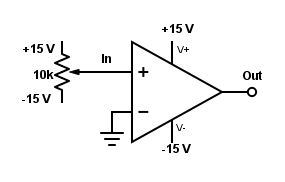
\includegraphics[scale=0.5]{Diagrams/c-a.png}
    \caption{Op-amp in a simple circuit, with no feedback loop. The potentiometer on the left serves as a variable DC voltage source.}
    \label{circuit:a}
\end{figure}

With no feedback loop and one of the inputs grounded, we expect to see an exceptionally large output signal (based on the exceptionally large output gain) that changes proportionally to changes in the input signal. By equation \ref{eqn:simpleGain}, only a zero input signal could result in a zero output signal.\\


\subsection{Results}

Using circuit \ref{circuit:a} we find that very small changes to the input signal cause the output signal to hit its limits at $\pm 15\ V$. This is consistent with the very large output gain we expect from this op-amp, and the output signal was consistently capped at $\pm 15\ V$ as expected based on our constant power supply to the amplifier.\\

We found that the circuit was far too sensitive to changes in the input signal for us to make an attempt at adjusting it manually to $0\ V$. Instead, by connecting both inputs to a common ground (reducing the voltage difference between them to 0), we found that the output signal also went to $0\ V$ as expected.\\


\section{Inverting Amplifier}
\subsection{Experimental}

One of the features of an op-amp is its two inputs--called the inverting and non-inverting inputs. In contrast with part 1, in part 2 we ground the non-inverting input and the circuit with a signal at the inverting input. As the name suggests, signals at this input are inverted at the output of the amplifier.\\

\begin{figure}[H]
    \centering
    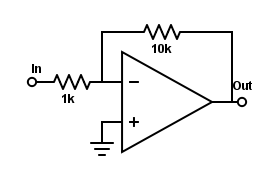
\includegraphics[scale=0.5]{Diagrams/c-b.png}
    \caption{In this circuit, the input signal is fed to the inverting input, and there is a feedback loop between the output and inverting input.}
    \label{circuit:b}
\end{figure}

Now that the circuit includes a feedback loop (in the form of a $10\ k \Omega$ resistor between the output and inverting input), we're required to do a little bit of extra analysis to find the expected output gain.\\

The second op-amp rule tells us that the inputs draw no current--so all of the current flowing through the $1\ k \Omega$ resistor must also be flowing through the $10\ k \Omega$ resistor. \\

% MATH: I_1k = I_10k
\begin{equation}
    I_{1k} = I_{10k}
\end{equation}

By applying Ohm's Law, we find that\\

% MATH: VIN - V_INVERTING / R_1k = V_INVERTING - VOUT / R_10k
\begin{equation}
    \frac{V_{In} - V_{-}}{R_{1k}} = \frac{V_{-} - V_{Out}}{R_{10k}}
\end{equation}

The first op-amp rule tells us that the difference between the inputs should be zero. Since the non-inverting input is grounded, we must assume that the circuit will react to make the voltage at the inverting input zero. Then,\\

% MATH: VIN / R_1k = -VOUT / R_10k
\begin{equation}
    \frac{V_{In}}{R_{1k}} = \frac{-V_{Out}}{R_{10k}}
\end{equation}

% MATH: VOUT = -R_10k / R_1k * VIN = -10 KILOHM / 1 KILOHM * VIN
\begin{equation}
    V_{Out} = \frac{-R_{10k}}{R_{1k}} V_{In} = \frac{-10\ k \Omega}{1\ k \Omega} V_{In}
\end{equation}

% MATH: VOUT = -10 VIN IMPLIES BETA = -10
\begin{equation}
    V_{Out} = -10\ V_{In} \Longrightarrow \beta = -10
\end{equation}

This negative-valued gain also confirms that we expect the output signal to be inverse of the input signal.\\


\subsection{Results}

For a $10\ Hz$ sine wave input, and powering the op-amp with $\pm 20\ V_{DC}$, we measured $V_{In} = 2.20\ V$ peak-to-peak, and $V_{Out} = 19.4\ V$ peak-to-peak for a gain of $8.82$. The output signal was also inverted, consistent with a negative (inverting) gain.\\

By returning our op-amp power to $\pm 15\ V_{DC}$, we found that the maximum output voltage swing was about $15\ V$, consistent with what we saw in the first part of the lab. \\

% PLOT: OUTPUT SIGNAL RESTRICTED BY VOLTAGE SWING
\begin{figure}[H]
    \centering
    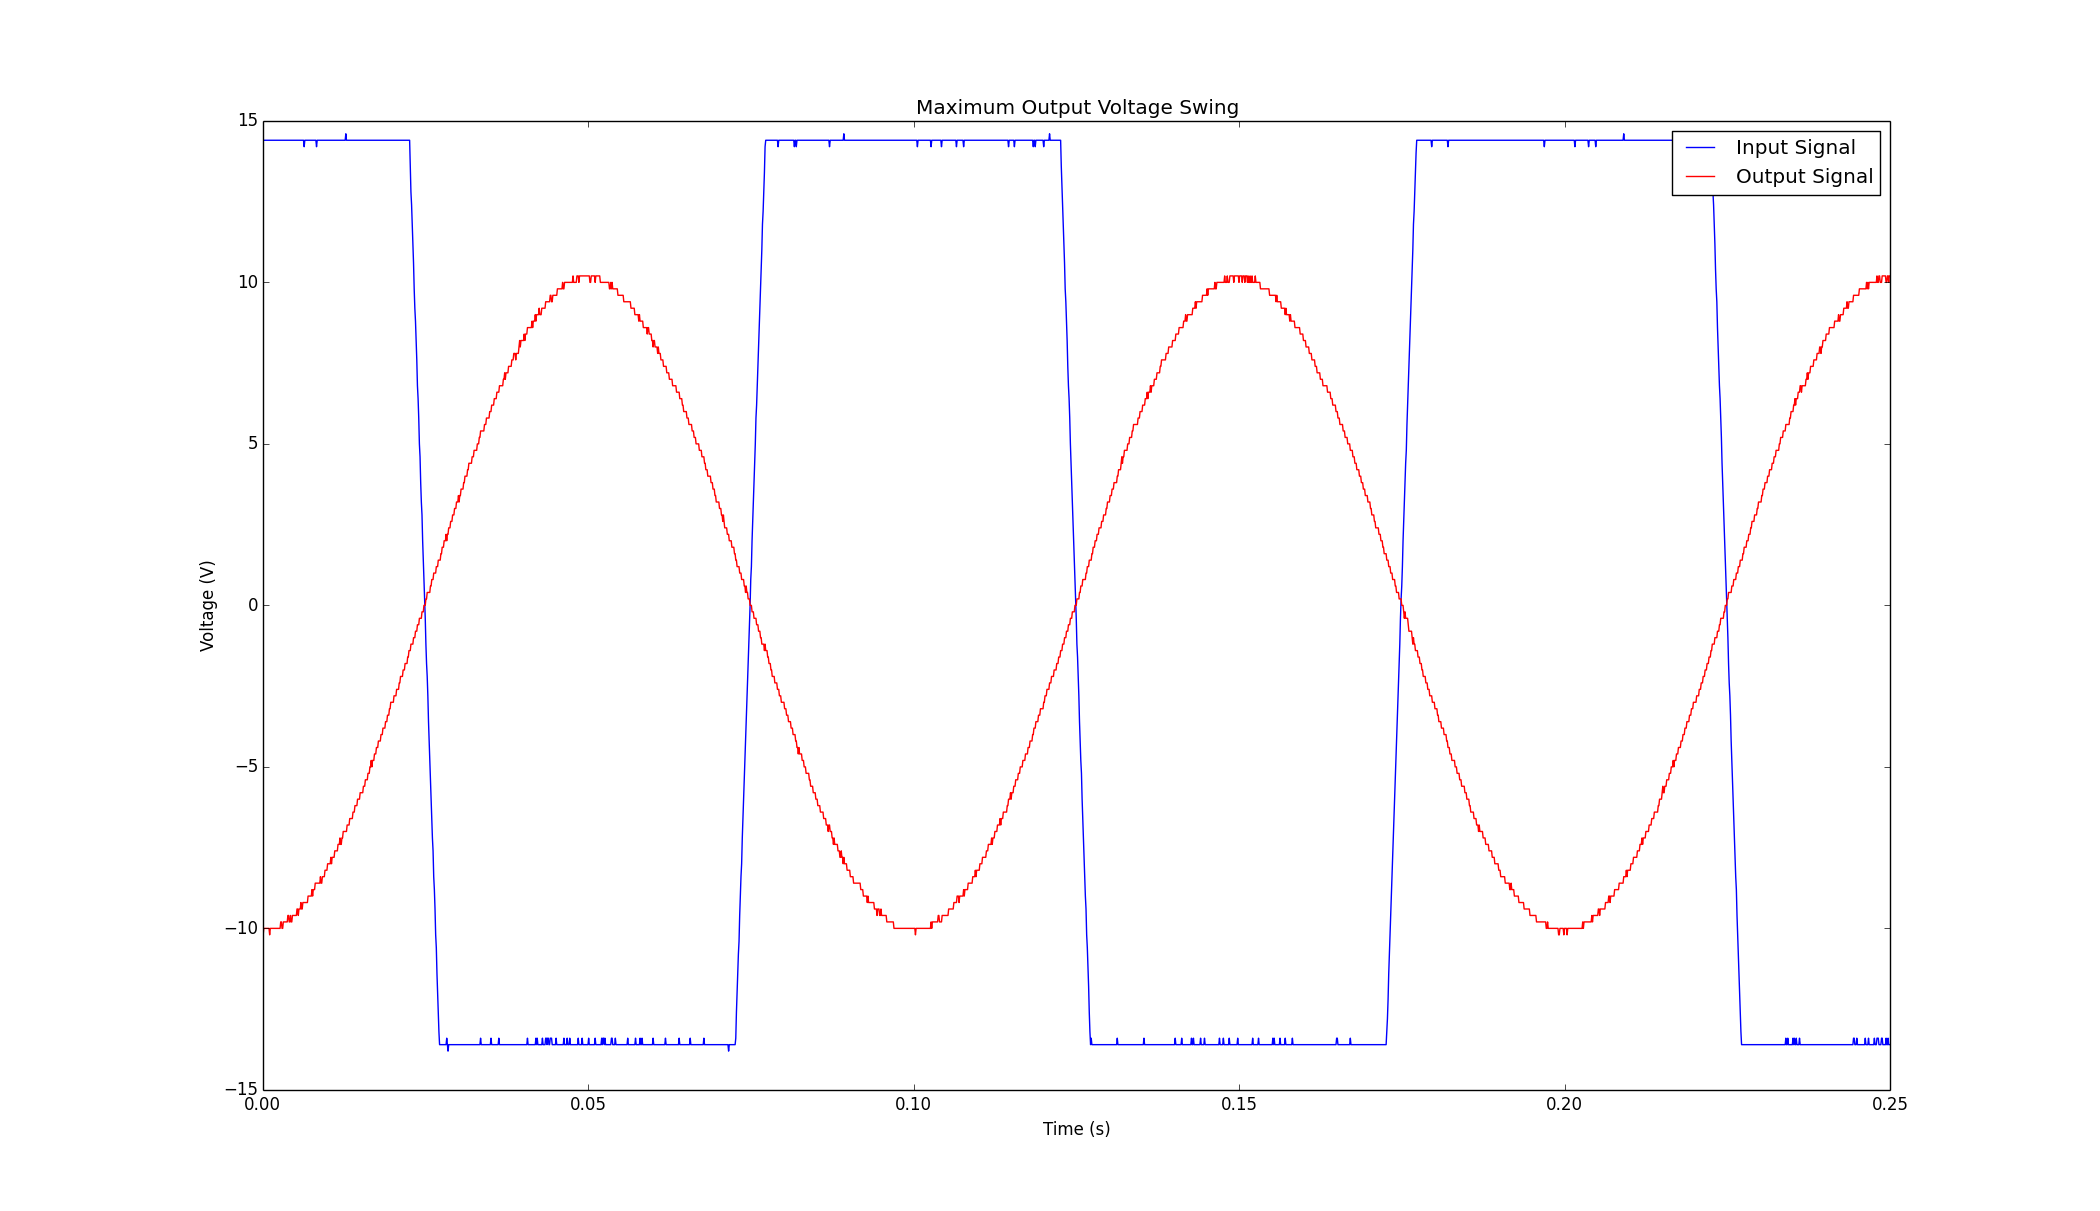
\includegraphics[scale=0.3]{Plots/figB.png}
    \caption{The flat regions at the peaks of the output signal show how the voltage swing is restricted by the DC voltage used to power the op-amp.}
    \label{fig:b}
\end{figure}

In observing the frequency-dependent behaviors of the output signal, we began to see some interesting effects at freqencies of $100\ kHz$, $1\ MHz$, and $5\ MHz$:\\

% TABLE: Theory Gain | Frequency | Output Type | Phase Shift? | DC Offset? | Measured Gain
\begin{center}
    \begin{tabular}[H]{ | c | c | c | c | c | c | }
        \hline
        Theory Gain & Input Frequency & Output Waveform & Phase Shifted? & DC Offset & Exp. Gain \\ \hline
        -10 & 100 kHz & Triangle & Yes & 0 & \textless 10 \\ \hline
        & 1 MHz & Triangle & Yes & Down & \textless 1 \\ \hline
        & 5 MHz & Sawtooth & Yes & Down & \textless 1 \\ \hline
        -100 & 100 kHz & Sine & Yes & Up & \textless 100 \\ \hline
        & 1 MHz & Sine & Yes & Up & \approx 1 \\ \hline
        & 5 MHz & Sine & Yes & Up & \textless 1 \\ \hline
        -1000 & 100 kHz & Sine & Yes & Up & \textless 1000 \\ \hline
        & 1 MHz & Signal too fuzzy to record data & & & \\ \hline
        & 5 MHz & Signal too fuzzy to record data & & & \\ \hline
    \end{tabular}
\end{center}

From these observations it appears that as the theoretical gain of the circuit increases (effectively, as the impedances grow larger), the phase shift and DC offset of the input signal increase. At higher frequencies, we see the output signal become smaller and more distorted.\\

It seems to me that the phase shift is a result of the input signal (or possibly the feedback signal) is passing through a resistor, and is "slowed down." The DC offset could be the result of a voltage difference across the resistor in the feedback loop, which is effectively a DC voltage added to the AC signal resulting in an amplitude shift. The distortion and diminished output gain are a little harder to explain.\\


\section{Non-Inverting Amplifier}
\subsection{Experimental}

In the part 3 of the lab, we use a circuit very similar to the one in part 2. Here, there are a couple of fundamental differences:

% CIRCUIT: c-c.png
\begin{figure}[H]
    \centering
    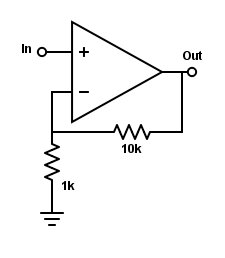
\includegraphics[scale=0.5]{Diagrams/c-c.png}
    \caption{Non-inverting amplifier circuit, with negative feedback.}
    \label{circuit:c}
\end{figure}

First and foremost, the circuit is non-inverting because we feed the input signal to the non-inverting input. We can verify this by calculating the expected gain of the circuit using the op-amp rules and Kirchoff's rules.

By the first rule, we know that the input voltages will be equal. We also know from the circuit diagram that the voltage at the non-inverting input will be equal to the voltage of the input signal:

\begin{equation}
    V_{-} = V_{+} = V_{In}
\end{equation}

We can also relate $V_{In}$ and $V_{Out}$ by using the voltage drop across the $10\ k \Omega$ resistor:

\begin{equation}
    V_{In} = V_{Out} - V_{10k}
\end{equation}

\begin{equation}
    V_{In} = V_{Out} - I R_{10k}
\end{equation}

After applying Ohm's Law, it's necessary to find the current through the $10\ k \Omega$ resistor. Fortunately, the second op-amp rule tells us that there is no current flowing to the inverting input--then, by Kirchoff's junction rule, the current through the $10\ k \Omega$ resistor must be the same as the current flowing through the $1\ k \Omega$ resistor. 

Then, using the voltage drop across that resistor:

\begin{equation}
    V_{In} - V_{1k} = 0
\end{equation}

\begin{equation}
    V_{In} = V_{1k} = I R_{1k} \Longrightarrow I = \frac{V_{In}}{R_{1k}}
\end{equation}

We can then use this definition for $I$ in the relationship between $V_{In}$ and $V_{Out}$:

\begin{equation}
    V_{In} = V_{Out} - V_{In} \frac{R_{10k}}{R_{1k}}
\end{equation}

\begin{equation}
    V_{Out} = V_{In} (1 + \frac{R_{10k}}{R_{1k}})
\end{equation}

\begin{equation}
    \beta = 1 + \frac{10\ k \Omega}{1\ k \Omega} = 11
\end{equation}

A positive gain indicates that the output we observe should not be inverted.

The other key difference between this circuit and the one from part 2 is that the resistors remain on the inverting side of the op-amp. Now, instead of forcing the input signal and feedback to flow on the same side of the circuit, they are flowing on opposite sides.


\subsection{Results}

Driving the circuit with a $1\ V$ peak-to-peak sine wave at $100\ Hz$, we measured $V_{In} = 2.2\ V$ peak-to-peak, $V_{Out} = 22.6\ V$ peak-to-peak, resulting in a gain of $\beta = 10.3$. This is reasonably close to the theoretical gain, $\beta = 11$.


\section{Follower}
\subsection{Experimental}


\end{document}
